\documentclass{article}
\usepackage{geometry,tikz}
\usetikzlibrary{shapes.geometric}
\geometry{paperwidth=15cm, paperheight=6cm,left=2pt,right=2pt,top=2pt,bottom=2pt}
\pagestyle{empty}
\begin{document}
\centering
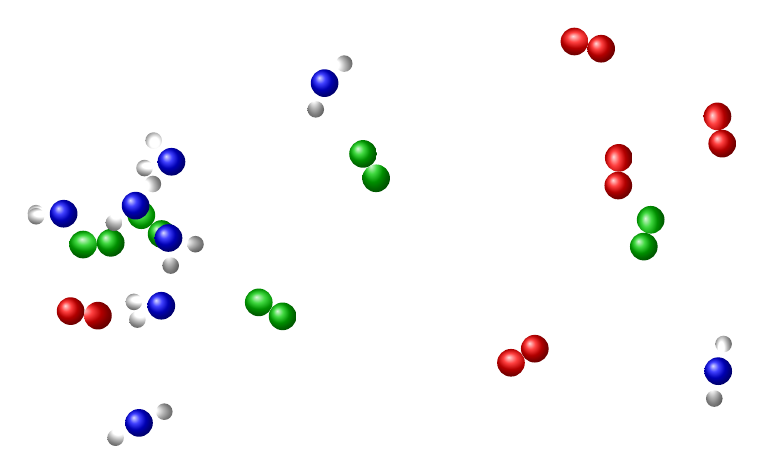
\begin{tikzpicture}
\foreach \typemol in {{green!80!black},red}
{
  \foreach \nmol in {1,...,5}
  {
    \shade[shading=ball,ball color=\typemol] (5*rand,2.5*rand) circle (5pt) coordinate (a1);
    \shade[shading=ball,ball color=\typemol] (a1) ++(360*rand:10pt) circle(5pt);
  }
}
\foreach \nmol in {1,...,8}
{
  \shade[shading=ball,ball color=blue] (5*rand,2.5*rand) circle (5pt) coordinate (a1);
  \shade[shading=ball,ball color=white] (a1) ++(360*rand:10pt) circle(3pt);
  \shade[shading=ball,ball color=white] (a1) ++(360*rand+119:10pt) circle(3pt);
}
\end{tikzpicture}
\end{document}
